% Archivo generado automáticamente con los problemas
\section*{Problems}
Sección: 32_Quantum_chromodynamics_and_the_parton_model
Páginas: 717-719
Contenido:
32.1 Derive an expression for the mean charge radius ⟨r2⟩=
!
d3x r2ρ(x) in terms of
a form factor F

q2
by expanding F

q2
=
!
d3x ei⃗q·⃗xV (x) around x = 0. What
is the mean charge radius of the proton from Eq. (32.9)?

32.2 Show that the PDFs, as classical probabilities, should satisfy 
j
!
dx xfj(x) = 1,
as in Eq. (32.29). [Hint: consider the average momentum for each parton.]

32.3 Derive the expansion in Eq. (32.38). One way to do this is to write
 1
0
dx x−1+εf(x) =
 1
0
dx x−1+εf(0)+
 1
0
dx x−1+ε [f(x) −f(0)] (32.118)
and to evaluate the first term and Taylor expand the second term.

32.4 Evaluate the relationship between W1 and W2 that would result instead of the
Callan–Gross relation if quarks were scalars. How could you test this prediction?

32.5 Calculate the g →gg splitting function by taking the collinear limit of gg →gg
scattering. You can use the cross section calculated in Chapter 27.

32.6 Find the limits of integration on z for t = p2
T in the process γ⋆→q¯qg discussed
in Section 32.3. Then calculate P(t) and the Sudakov factor Δ(Q, t) explicitly.
Repeat the exercise for t = m2 and t = θ. Which part of the Sudakov factor is
universal?

32.7 In this problem, you will show that Q →∞at fixed ω = 2P ·q
Q2 or equivalently fixed
χ ≡2mp
ω
implies that J(xμ)J(0) is dominated by the lightcone, where x2
μ →0.
(a) In the proton rest frame, show that
qμxμ = ωQ2
2mp
(x0 −r) −mp
ω r + O
1
Q2
,
(32.119)
where r ≡⃗q·⃗x
|⃗q| .
(b) Use the method of stationary phase to show that at fixed ω, W μν, in the form
of Eq. (32.78), is dominated by
x0 −r
≤
c1
Q2 and r ≤c1 for two constants
c1 and c2 as Q →∞.
(c) Show that x2 ≤const
Q2 and therefore that J(xμ)J(0) is dominated by lightlike
separations in the DIS limit.

32.8 Relating imaginary parts to discontinuities. The goal of this problem is to verify
Eq. (32.83).
(a) By expanding the time ordering in terms of θ(t) and θ(−t) show that T μν as
in Eq. (32.81) can be written as
Tμν(ω, Q) =
X
(2π)3δ3(⃗pX −⃗q −⃗P)
p0
X −p0 −q0 −iε
⟨p+|Jμ(0)|X⟩⟨X|Jν(0)|p+⟩
+
X
(2π)3δ3(⃗pX + ⃗q −⃗P)
p0
X −p0 + q0 −iε
⟨p+|Jμ(0)|X⟩⟨X|Jν(0)|p+⟩.
(32.120)
You may want to use θ(t) =
1
2πi
! ∞
−∞
ds
s−iεeist.
Problems
699
(b) Use part (a) to show that one of the terms above does not contribute to the
discontinuity in the physical region and that Wμν = −i Disc Tμν.

32.9 Show that current conservation implies a sum rule for each flavor in QCD using
spin-1 operators in the OPE, as we did for spin 2 in Section 32.4.4.

32.10 Show that p2
T =
ˆsˆtˆu
(ˆs+Q2)2 and verify Eq. (32.58).

32.11 Relate the lightcone PDF definition from Eq. (32.117) to the Mellin moments
from Section 32.4.4.
(a) Compute the m = 1 moment of the lightcone PDF definition to show that you
get the matrix element of the spin-1 operator ˆOμ
q = ¯ψγμψ. Be careful with the
limits of integration.
(b) Show that you can reproduce the matrix elements of the twist-2 spin-m
operators by taking moments.
(c) Can you construct the lightcone PDF definition from the Mellin moments?

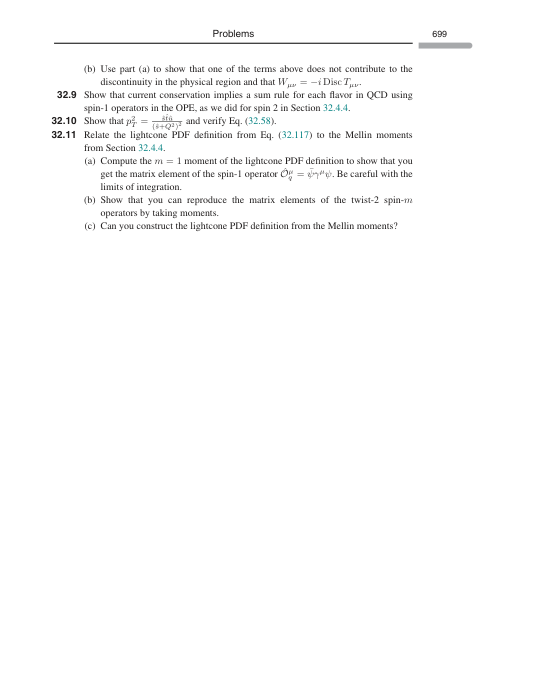
\includegraphics{./figs/32_Quantum_chromodynamics_and_the_parton_model_page_719.png}

---

